\subsection{Problemstellung}

Zur Umsetzung des WebApp-Wrappers werden die beiden Frameworks Capacitor und Electron verwendet.
Diese beiden Frameworks bieten eine Reihe von Vorteilen, darunter eine einfache Handhabung, eine weite Verbreitung, einfache Erweiterungsmöglichkeiten und die Möglichkeit, Anwendungen mit \ac{html}, \ac{css} und JavaScript zu erstellen.
\cite{capacitor:docs, electron:docs}

Beide Frameworks haben jedoch auch ihre Grenzen.
Electron-Anwendungen können nur für Desktop-Plattformen (Windows, Linux und macOS) kompiliert werden.
Das Electron Framework bieten dafür jedoch folgende Funktionen, die für den WebApp-Wrapper benötigt werden.
\cite{electron:docs}

\begin{itemize}
    \setlength\itemsep{-0.5em}
    \item Externe Webinhalte können in einem Fenster über bestimmte Bereiche der Benutzeroberfläche gelegt werden.
    \item Node.js Projekte können eingebunden werden, um den Funktionsumfang der Anwendung zu erweitern.
\end{itemize}

Capacitor-Anwendungen können hingegen für Mobile"=Plattformen (Android und iOS) kompiliert werden.
Das Framework bietet außerdem die Möglichkeit, diese Anwendungen mithilfe von Electron auch für Desktop"=Plattformen zu kompilieren.
Das ermöglicht das Erstellen von Anwendungen, die auf allen gängigen Plattformen ausgeführt werden können.
Allerdings bietet Capacitor nicht den gleichen Funktionsumfang wie Electron.
\cite{capacitor:docs, capacitor-electron}

\begin{figure}[H]
    \centering
    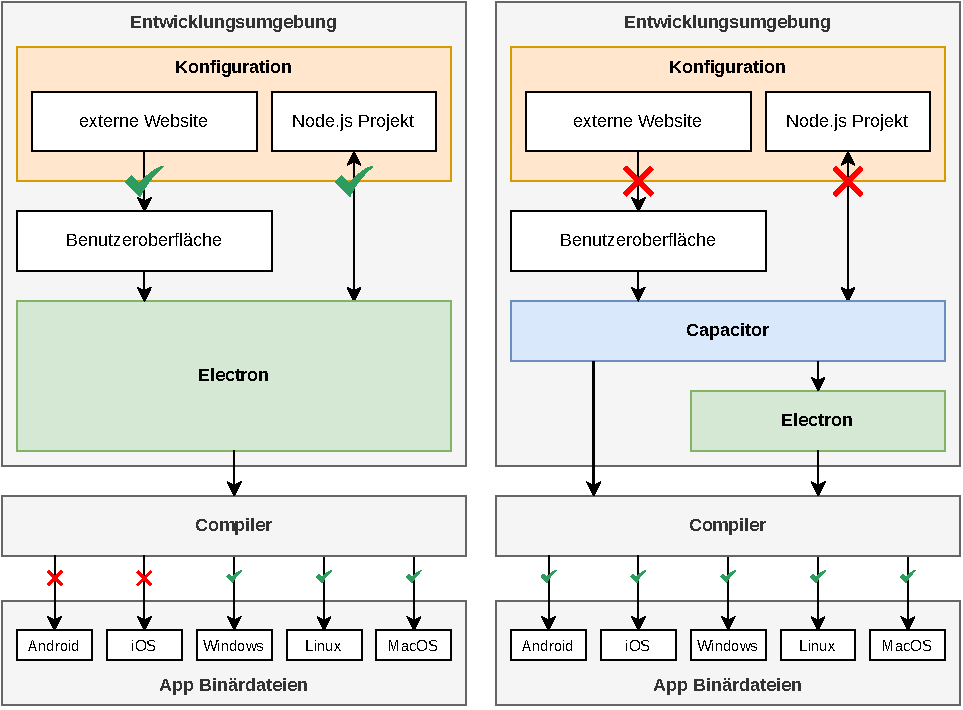
\includegraphics[width=\textwidth]{assets/01_Einführung/03_Problemstellung.drawio.pdf}
    \caption{Problemstellung}
\end{figure}

Daher ist es aktuell nicht möglich, eine Anwendung mit \ac{html}, \ac{css} und JavaScript zu erstellen, die externe Webinhalte anzeigen kann, ein zusätzliches Node.js Projekt einbinden kann und sowohl auf Desktop- als auch auf Mobile"=Plattformen funktioniert.

Aus den beschriebenen Problemen lassen sich jedoch zwei mögliche Lösungsansätze ableiten:

\begin{enumerate}
    \setlength\itemsep{-0.5em}
    \item
    Das Electron Framework wird modifiziert, um es für Mobile"=Plattformen kompatibel zu machen.
    Dies würde jedoch wahrscheinlich eine tiefgreifende Änderung des Frameworks erfordern, da Mobile"=Plattformen und Desktop"=Plattformen sehr unterschiedlich aufgebaut sind.
    \item
    Das Capacitor Framework wird erweitert, um die fehlenden Funktionen hinzuzufügen.
    Dies ist eine einfachere Lösung, da Capacitor bereits für Mobile"=Plattformen kompatibel ist und eine Electron"=Unterstützung bietet, um auch Desktop-Plattformen zu unterstützen.
\end{enumerate}

Aufgrund der Komplexität des ersten Lösungsansatzes wurde der zweite Ansatz gewählt.
Infolgedessen sollen zwei Erweiterungen für das Capacitor Framework entwickelt werden:

\begin{itemize}
    \setlength\itemsep{-0.5em}
    \item \textbf{Capacitor-NodeJS:} Diese Erweiterung soll eine Node.js Runtime bereitstellen, um Node.js Projekte in Capacitor Anwendungen einzubinden.
    \item \textbf{Capacitor-BrowserView:} Diese Erweiterung soll eine WebView Unterstützung zu Capacitor hinzufügen, um externe Webinhalte in einem Fenster über bestimmte Bereiche der Benutzeroberfläche legen zu können.
\end{itemize}

Die Erweiterungen werden im Kapitel \hyperref[sec:Capacitor-NodeJS]{Capacitor-NodeJS} und \hyperref[sec:Capacitor-BrowserView]{Capacitor-BrowserView} näher erläutert.

Durch diese Erweiterung des Capacitor Frameworks können die fehlenden Funktionen ergänzt werden.
Damit ist es möglich, den WebApp-Wrapper zu realisieren, der das Hauptziel dieser Arbeit darstellt.
